\chapter{Contexte et problématique}



\section{Principes généraux}

%test \citealt{ref4}


A l'heure actuelle, le logiciel SIEL permet d'effectuer un certain nombre de traitements bien définis dans le contexte de la désertification et des risques de dégradation du sol. Le contexte environnement-santé est également une des préoccupations de l'UMR Espace-Dev et la réutilisation de cet outil, pour la création d'indicateurs du risque de transmission de maladies infectieuses, nous a apparu particulièrement intéressante. Afin d'optimiser et de généraliser cette réutilisabilité, il faut penser les chaînes de traitements dans ce nouveau contexte. \\

De plus, le SIEL est disponible en tant que plugin ArcGIS  et fonctionne avec des séries de traitements et d'opérations ciblées sur le type d'indice à produire. L'objectif à long terme est de retravailler ce logiciel pour qu'il devienne plus modulaire et générique, de préférence dans un contexte "Open Source". Nous avons donc décidé d'ouvrir l'outil et à repenser son architecture dans un contexte Open Source. \\

Dans ce contexte, la conception et le développement d'une chaîne de traitements liés aux indices santé-environnement avaient comme objectif de servir d'expérience préliminaire à la conception et à la réalisation d'une nouvelle architecture informatique du logiciel. %Le développement d'un \textbf{logiciel ouvert} a permis de franchir une étape supplémentaire dans le développement informatique du SIEL.
L'intégration de la création automatisée d'indicateurs dans le domaine environnement-santé constituera de plus, une première piste dans l'objectif plus large qui consiste à faire du SIEL un outil générique adaptable à divers autres contextes comme par exemple la déforestation.\\

Nous allons maintenant présenter brièvement le SIEL, ses principes, son architecture informatique et la chaîne de traitements qu'il exécute. Par la suite les problématiques du présent stage seront expliquées en détail.\\



%La définition des facteurs de risque est une autre étape indispensable de la conceptualisation et de l'élaboration de la chaîne de traitements. A partir d'un modèle du cycle de la malaria, des modèles de données et de traitements permettront de dégager les étapes nécessaire pour aboutir au résultat souhaité: un prototype d'une chaîne de traitements permettent de créer des cartes de risques du paludisme. A partir des données d'entrée choisies par l'utilisateur la chaîne calculera automatiquement les zones à risque de transmission du paludisme. Les résultats seront représentés sous forme de cartes.


\section{Le logiciel SIEL}

Le SIEL est un logiciel qui instrumente un modèle environnemental \citep{Loireau2007} spatialisant les pratiques d'exploitation des ressources sur un territoire, modélisant les paysages et évaluant les risques de dégradation des ressources.\\

Le SIEL est un outil conçu pour répondre aux besoins des scientifiques et décideurs concernés par la lutte contre la dégradation et la gestion des ressources naturelles. Le SIEL est capable d'anticiper les risques et de les suivre, ce qui est important notamment dans le cadre de la mise en place d'observatoires. Cet outil donne également la capacité aux scientifiques et aux décideurs de mesurer l'impact des opérations déjà effectuées sur un territoire et d'optimiser les actions futures notamment en terme de gestion des ressources  \citep{SIEL2012}.\\ 

Le logiciel a été conceptualisé à partir de 1993 par Maud Loireau dans le cadre de sa thèse. En même temps un premier prototype a été développé. En 2000, dans le cadre de la lutte contre la désertification, la démarche scientifique et le modèle général du SIEL ont été adoptés par le programme ROSELT \footnote{Réseau d'observatoires de Surveillance Ecologique à Long Terme} de l’OSS \footnote{Observatoire du Sahara et du Sahel}. Ceci a permis de développer un premier logiciel SIEL qui couvrait l'ensemble de la chaîne de traitements proposée. Une première version du logiciel traitant la ressource « végétation » a pu être déployée dans le réseau ROSELT/OSS dès la fin de l'année 2003.
A partir de 2006, les différents acteurs ont poursuivi les développements du logiciel. Ceci a débouché sur un logiciel opérationnel et prêt à être diffusé, une documentation (guide d'utilisateur, aide en ligne), une documentation technique (guide développeur, dictionnaire des données), une base de données exemple et des supports de formations. Actuellement, l'objectif principal reste le développement informatique du logiciel et le responsable du projet informatique est depuis 2010 Bertrand Guerrero.

%\subsection{Le "modèle" SIEL}
%
%
%Le SIEL se base sur le fonctionnement interactif milieux/sociétés sur un territoire dans lequel des acteurs, selon leurs représentations de leur territoire et leurs usages (agricole, pastoral, forestier), ont des pratiques qui permettent d'exploiter des ressources naturelles (physiques, biologiques) sur un territoire donné (Guide utilisateur). Les interactions entre l'espace, les acteurs, les usages et les ressources produisent des paysages qui vont composer les territoires. Ces paysages évoluent en fonction des interactions entre facteurs naturels et humains. 
%Pour mettre en œuvre ce phénomène, le modèle SIEL décompose le territoire en
%Unités Spatiales dites « de Référence » (USR). Ces USR correspondent à une délimitation
%spatiale des différents paysages du territoire par voie de modélisation.\\
%
%Un minimum de données est nécessaire pour alimenter la chaîne de traitements: 
%\begin{itemize}
%\item données socio-économiques (acteurs, stratégies, pratiques d'exploitation...)
%\item données biophysiques (ressources, végétation...)\\
%\end{itemize}
%
%Enfin, le modèle SIEL met en œuvre une méthode spatiale interdisciplinaire qui permet une cartographie dynamique des paysages et le calcul d'indices environnementaux associés \citep{Loireau2007}. 


\subsection{Architecture SIEL}

Le SIEL se présente sous forme d'un plugin ArcGIS et se base sur deux modules propriétaires:\\

\begin{itemize}
\item Module données (Logiciel Microsoft Access \textbf{SGBD}, langage de programmation : Visual Basic for Application (VBA)) pour la gestion et le stockage des tables attributaires (format .mdb).
\item Module SIG (Logiciel: ArcGIS Desktop avec l'extension Spatial Analyst, langage de programmation: Visual Basic 6.0 et langage ESRI ArcObjects) pour la gestion et le stockage des couches géographiques et les géotraitements.\\
\end{itemize}

Le système d'exploitation supporté est Windows XP, les logiciels supportés sont "Microsoft Office 2003" et "Microsoft Office 2007" pour le module données et "ArcGIS 9.1" et "ArcGIS 9.3" pour le module SIG. Les deux modules sont donc basés sur des outils propriétaires. Le SIEL a été développé en Visual Basic, langage informatique qui n'est plus supporté par les nouvelles versions d'ArcGIS ce qui cause un certain nombre de restrictions par rapport à son utilisation et le développement futur.

\subsection{Les chaînes de traitements du SIEL}

Les deux modules (Données et SIG), en faisant différents traitements, créent des \textbf{indices environnementaux spatialisés} qui permettent la cartographie des risques de dégradation des ressources. Les données utilisées et les résultats sont stockés dans une base de données Microsoft Access. 
% attention dire que ici on utilise le formalisme de Yuan et mettre ce formalisme 
% ensuite présenter les 3 chaines 
\begin{figure}[H]
\begin{center}
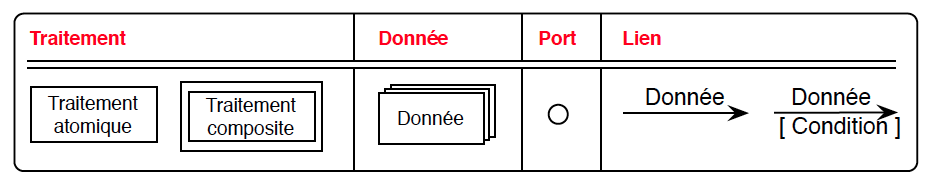
\includegraphics[width=16cm]{LinGraphique}\\
\caption{\label{LinGraph} Langage graphique proposé par Yuan Lin \citep{Lin2011}}
\end{center}
\end{figure}
A ce stade, nous utiliserons, pour formaliser les chaînes de traitements, le formalisme défini par Yuan Lin (cf. fig \ref{LinGraph}).

\paragraph{Description générale\\}

Le schéma \ref{SIEL1} explique de façon très simplifié le fonctionnement du SIEL. A partir de données statistiques et de données vectorielles le SIEL exécute des chaînes de traitements et fournit en sortie des indices de risque multi-usage.

\begin{center}
\begin{figure}[h] \centering
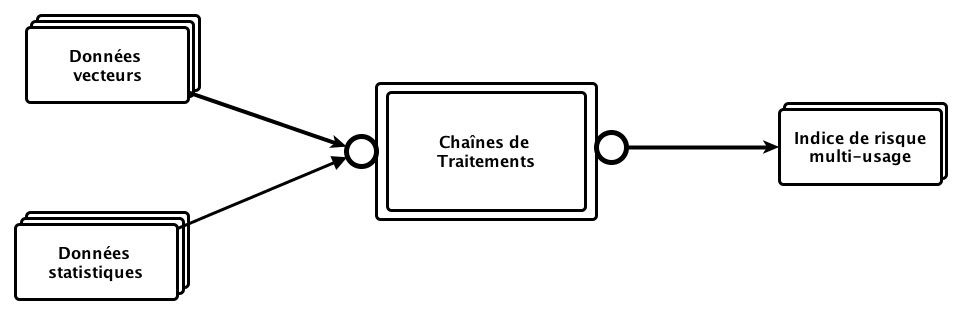
\includegraphics[width=16cm]{TraitementsSiel1.png}\\
\caption{\label{SIEL1} Description générale du SIEL}
\end{figure}
\end{center}

\paragraph{Chaîne de traitements abstraite\\}

Les traitements du SIEL peuvent être divisées en plusieurs sous-catégories: 

\begin{itemize}
\item Les traitements liés au territoire d'exploitation potentiel \footnote{Aire potentielle d’exploitation des ressources naturelles par un ou plusieurs groupes d’agents autour d’un centre d’activités, pour une période d’observation donnée. \citep{SIEL2012}}
\item Les traitements liés aux unités spatiales de référence \footnote{Une Unité Spatiale de Référence (USR) correspond à une délimitation spatiale d’un paysage par voie de modélisation \citep{SIEL2012}}
\item Les traitements liés aux indices de risque multi-usages

\end{itemize}

Les données d'entrée du SIEL sont des données vecteurs et des données statistiques. Au cours de l'exécution de la chaîne, des données intermédiaires sont également créées (au format raster, vecteur et statistique). 

\begin{center}
\begin{figure}[h] \centering
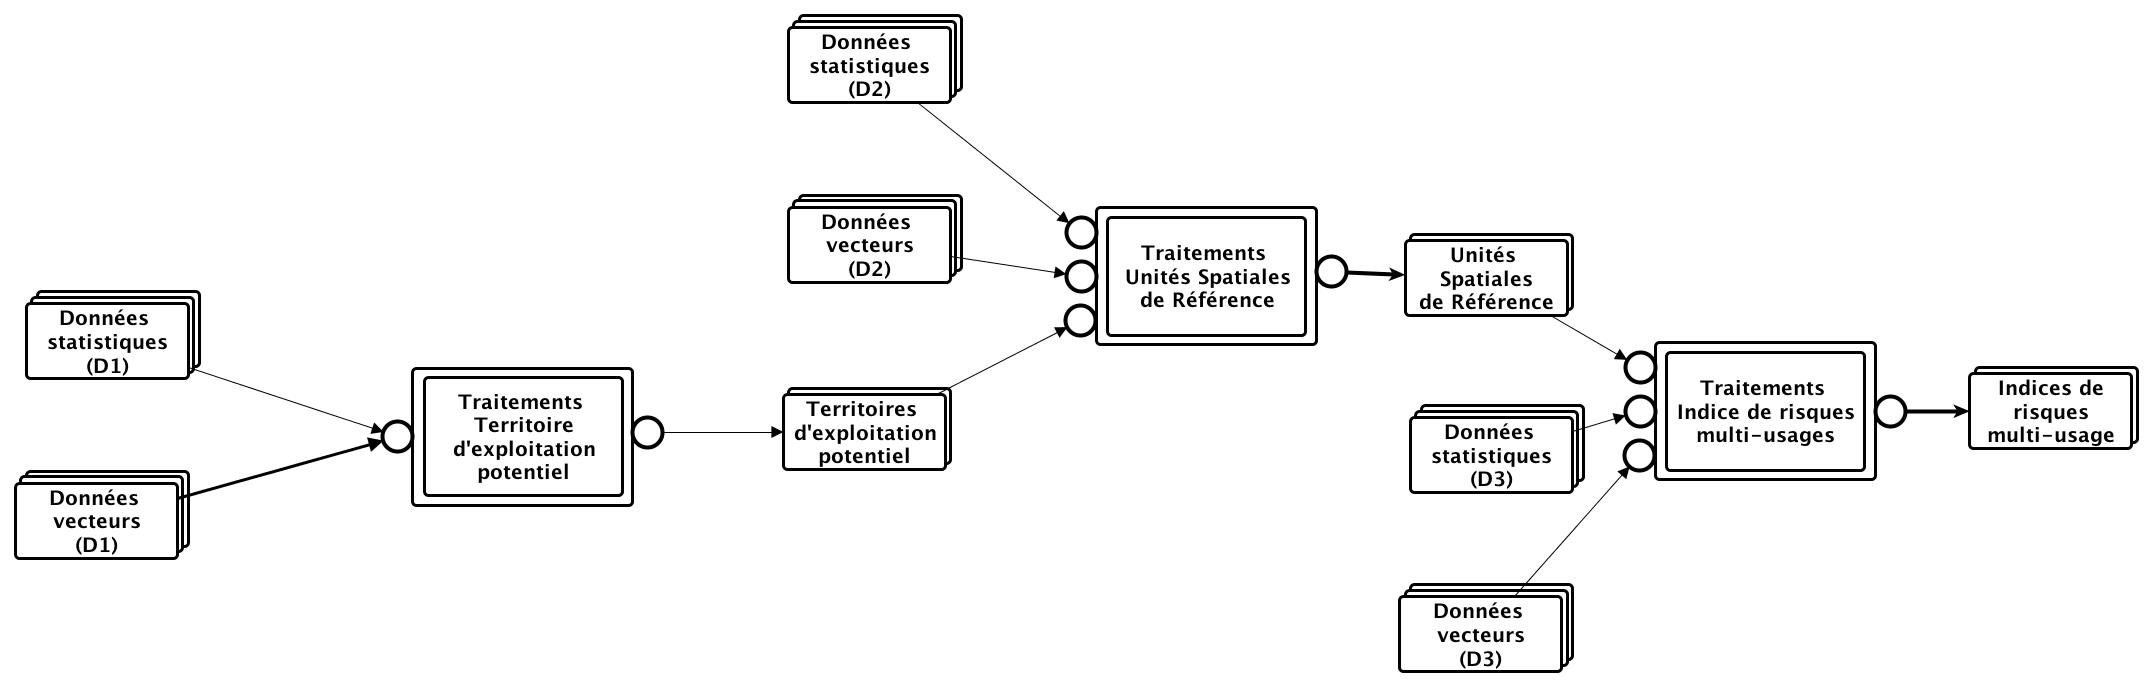
\includegraphics[width=16cm]{traitementsSiel2.png}\\
\caption{\label{SIEL2} Chaîne abstraite du SIEL}
\end{figure}
\end{center}

\newpage

\paragraph{Chaîne de traitements abstraite avec traitements élémentaires\\}

Le SIEL délimite dans un premier temps les territoires d'exploitation potentiels. Par la suite, le calcul des besoins et la spatialisation des pratiques permettent de délimiter les pratiques sur le territoire et plus précisément, à partir d'une intersection avec les unités paysagères, de créer des unités spatiales de référence.\\

A partir de différentes données d'entrée, le SIEL spatialise les prélèvement ce qui permet de déterminer les prélèvements en fonction de l'usage et de l'aire. Ce résultat temporaire et les unités spatiales de référence permettent finalement de calculer les indices de risque multi-usage en analysant l'usage par rapport aux prélèvements.

Les figures \ref{SIEL3} et \ref{SIEL4} montrent les traitements élémentaires du SIEL.





\begin{landscape}
\begin{figure}[h] \centering
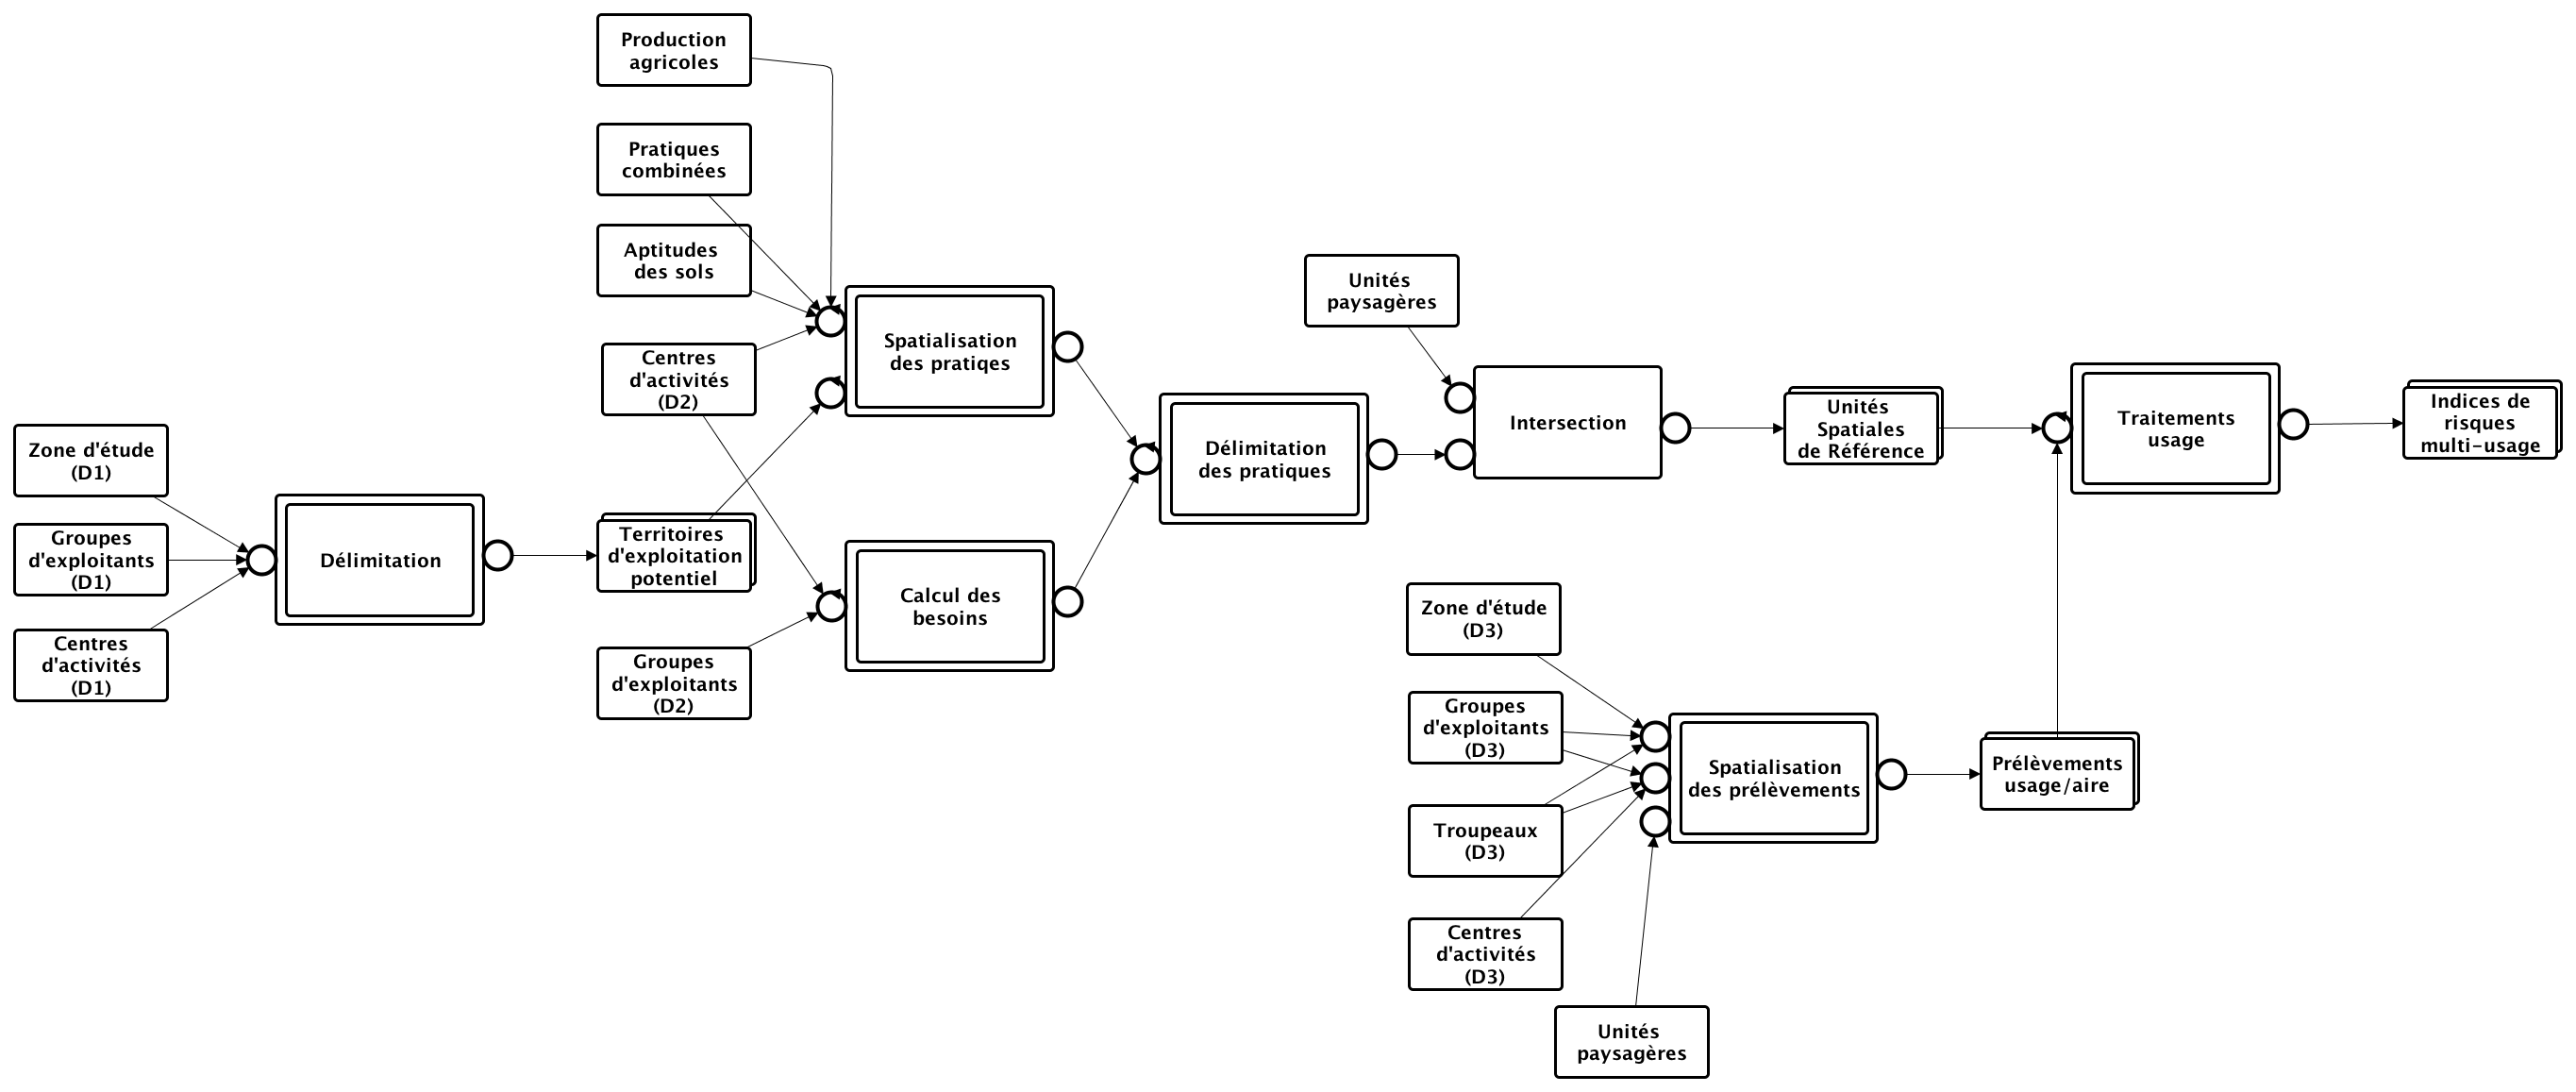
\includegraphics[width=23cm]{traitementsSiel3.png}\\
\caption{\label{SIEL3} Chaîne abstraite avec traitements élémentaires du SIEL}
\end{figure}
\end{landscape}

\begin{landscape}
\begin{figure}[h] \centering
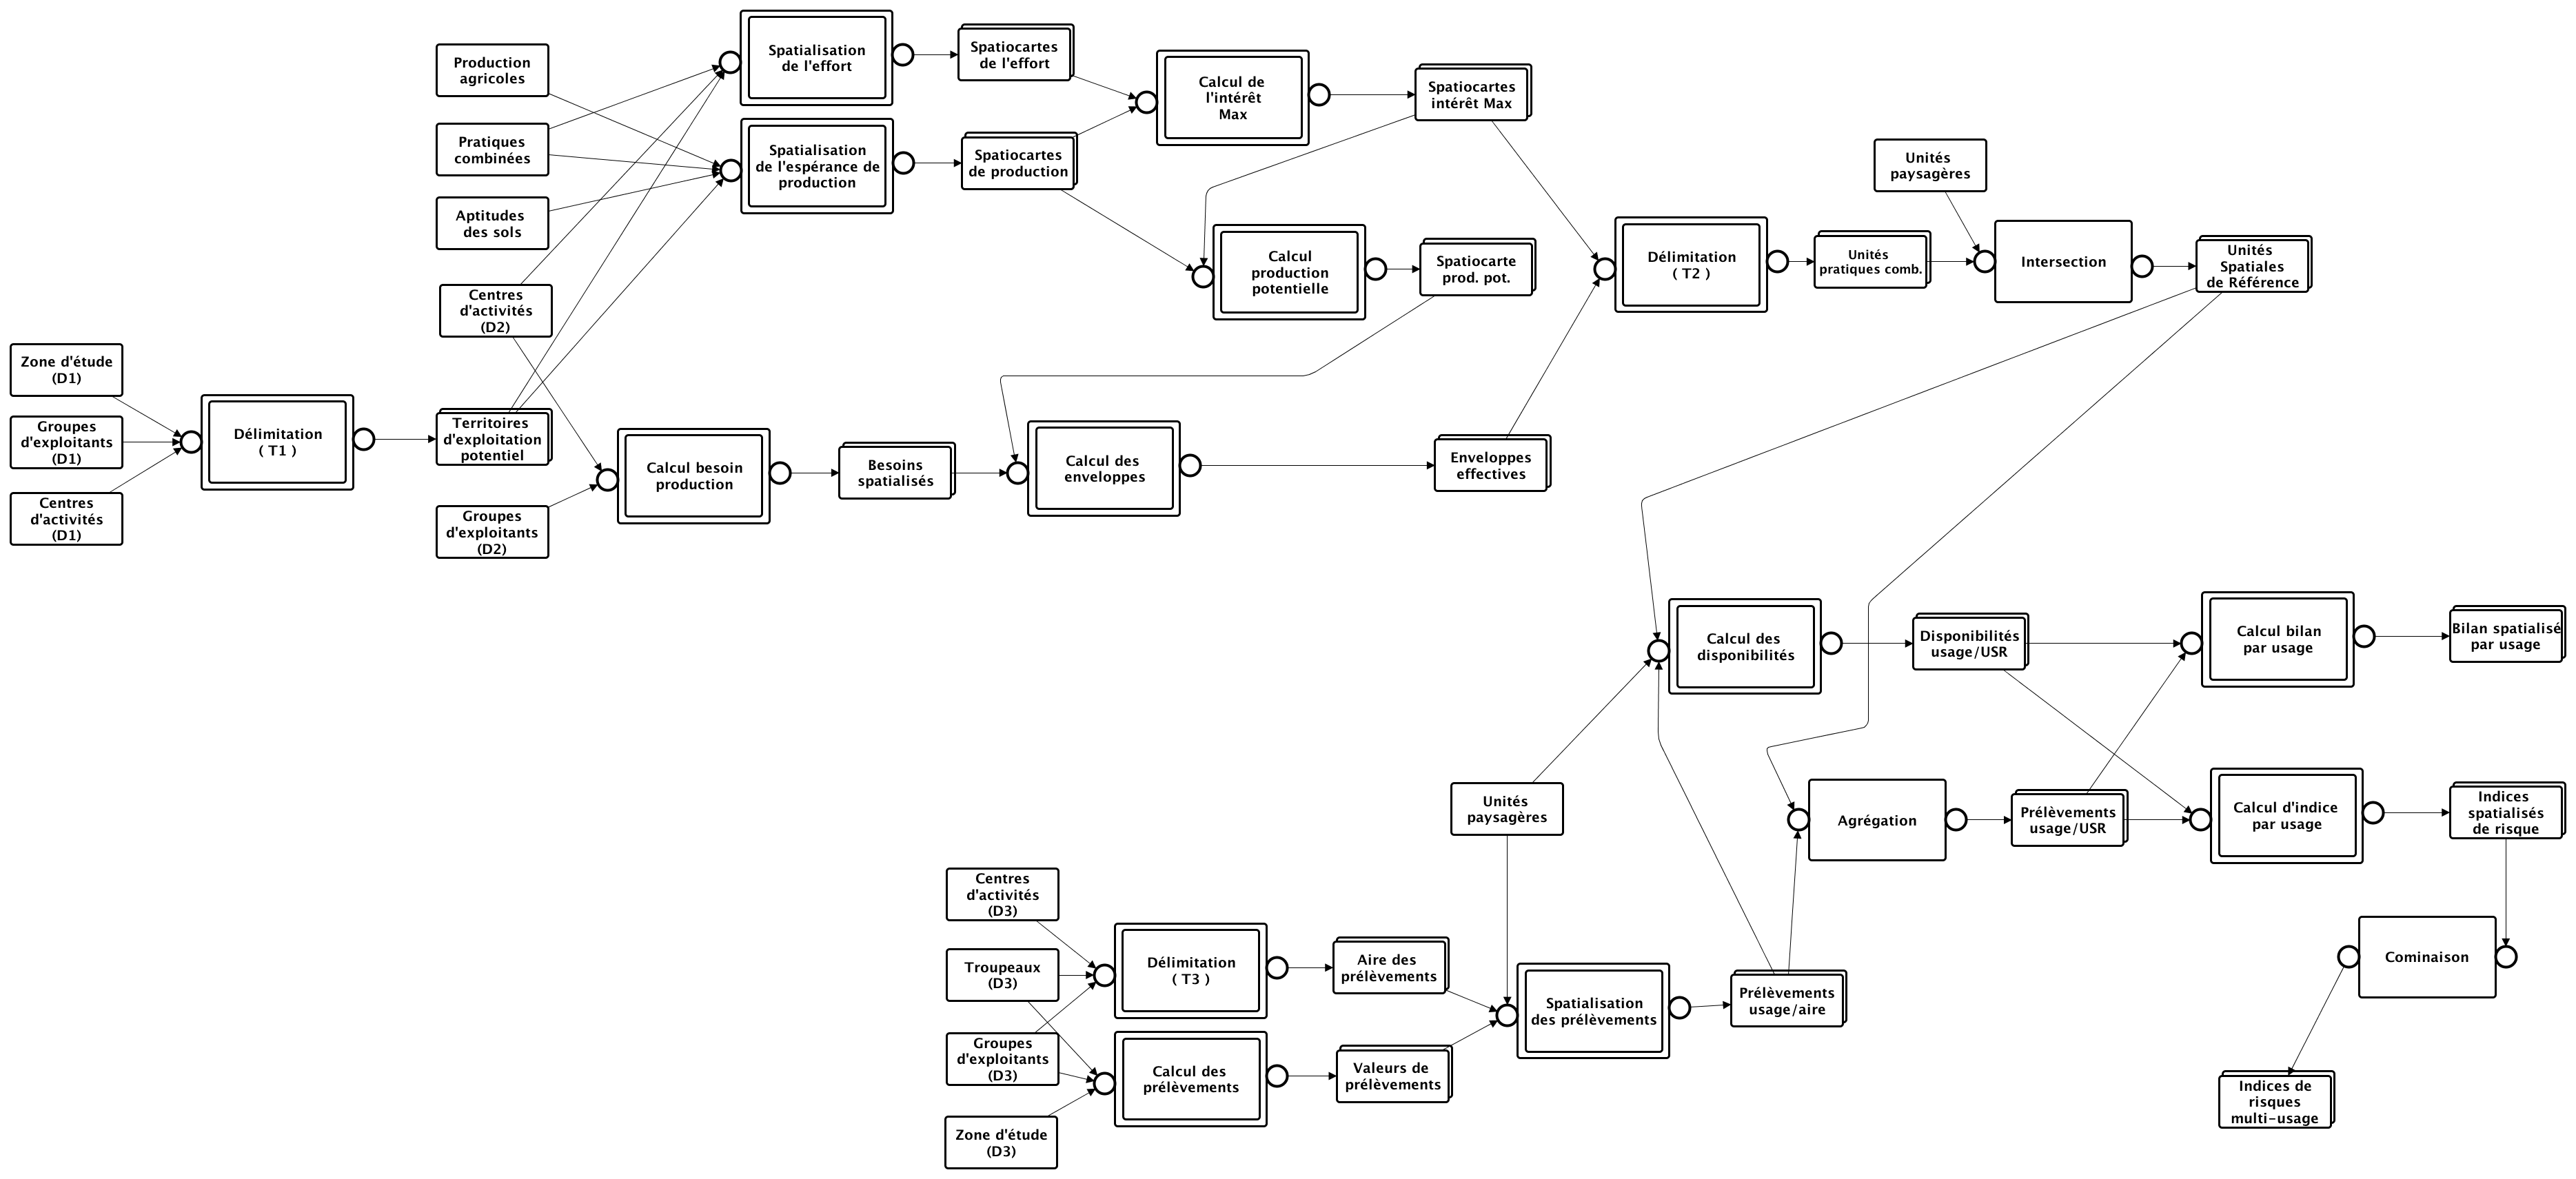
\includegraphics[width=23cm]{traitementsSiel4.png}\\
\caption{\label{SIEL4} Chaîne abstraite de plus en plus détaillée}
\end{figure}
\end{landscape}




%Suivi de phénomènes naturels ou anthropiques et l'orientation qui est choisi est de fabriquer des cartes révélatrices d'indicateurs pertinents.
%Exemple: désertifiaction (vulnérabilité à la désertification), déforestation
%Pour l'instant ce logiciel est un plugin ArcGIS et fonctionne avec des séries de traitements ou d'opérations ciblés sur le type d'indicateur à produire.

\newpage
\section{Problématiques du stage}


Étant donné la pluridisciplinarité du sujet de stage, les problématiques se regroupent en 2 catégories :\\
\begin{itemize}
\item Problématiques environnement-santé : Paludisme et les facteurs de risque de transmission
\item Problématiques informatiques : Conceptualisation des chaînes de traitements dans le contexte environnement-santé, choix de l'architecture et implémentation des outils (chaîne de traitements et logiciel ouvert).\\
\end{itemize}


Concernant le thème 'environnement-santé', la problématique principale est la compréhension du phénomène, la définition des facteurs de risque et la formalisation des éléments nécessaires à la mise en œuvre de la chaîne de traitements.\\

Au niveau informatique les points à traiter relèvent du choix de l'architecture informatique et de la réalisation d'un prototype de chaîne de traitements. Les principes de réutilisation et de généricité nous amènent à réfléchir sur une architecture "boîte blanche", qui consiste à ouvrir la boîte de la chaîne de traitements et à la déstructurer en boîtes élémentaires réutilisables. Le logiciel "ouvert" ainsi obtenu, permettra d'exécuter chaque traitement de la chaîne indépendamment les uns des autres et à les combiner selon les besoins de l'utilisateur.\\


%Le travail de Nadine Dessay sur l'élaboration de cartes de risques de paludisme va servir comme base lors de la définition des traitements à réaliser. Dans ce travail, elle définit les étapes nécessaires pour l'élaboration de ce type de cartes par rapport à la problématique du paludisme. Ces traitements sont réalisés sous ArcGIS, l'objectif est de trouver des fonctionnalités similaires avec des outils "OpenSource" et d'automatiser l'exécution de tous ces traitements et calculs à l'intérieur de la chaîne de traitements. Le logiciel ouvert permettra d'exécuter chacun de ces traitements indépendamment. \\
%
%
%Nadine Dessay a également extraits plusieurs données à partir d'une image de haute résolution \textbf{Quickbird} (...résolution) de la ville de Bandiagara au Mali qui serviront comme "données d'essai" pour le prototype de la chaîne de traitements.\\

En résumé la problématique générale du stage se dégage :\\ \textbf{Conceptualisation et développement d'outils pour cartographier des indicateurs relatifs à divers risques environnementaux.}
%
%L'idée est d'élargir les potentialités de cet outil afin de construire des indicateurs dans un contexte environnement-santé et de rendre le fonctionnement de cet outil plus souple, plus ouvert et donc faciliter son usage et son adaptation à divers contextes.


